\documentclass[a4paper,12pt,onecolumn]{article}

\usepackage[utf8]{inputenc}
\usepackage[english]{babel}
\usepackage{amssymb,amsmath,amsthm,array,epsfig,a4,verbatim,pstricks,url,subfig,
hyperref}

\newenvironment{keywords}{{\upshape\bfseries Key words. }\ignorespaces}{}

\newtheorem{thm}{Theorem}
\newtheorem{lem}{Lemma}

\newcommand{\R}{{\mathbb R}}
\newcommand{\spa}{\operatorname{span}}
\newcommand{\vol}{\mathcal{L}^d}
\newcommand{\dH}[1]{\;{\rm d}{\cal H}^{#1}} % Hausdorff measure
\newcommand{\dL}[1]{\;{\rm d}{\cal L}^{#1}} % Lebesgue measure
\newcommand{\bigchi}{\ensuremath{\mathrm{\mathcal{X}}}}
\newcommand{\charfcn}[1]{\bigchi_{#1}} % characteristic function
\newcommand{\Vh}{\underline{V}(\Gamma^m)}
\newcommand{\Wh}{W(\Gamma^m)}
\newcommand{\Vht}{\underline{V}(\Gamma^h(t))}
\newcommand{\Wht}{W(\Gamma^h(t))}
\newcommand{\uspace}{\mathbb{U}}
\newcommand{\pspace}{\mathbb{P}}
\newcommand{\kspace}{\mathbb{K}}
\newcommand{\xspace}{\mathbb{X}}
\newcommand{\sigmaO}{o}
\newcommand{\nabs}{\nabla_{\!s}}
\newcommand{\Id}{I\!d}
\newcommand{\id}{\rm id}
\newcommand{\ddt}{\frac{\rm d}{{\rm d}t}}
\newcommand{\NbulkT}{\vec{N}_{\Gamma,\Omega}^T}
\newcommand{\Nbulk}{\vec{N}_{\Gamma,\Omega}}
\newcommand{\errorXx}{\|\Gamma^h - \Gamma\|_{L^\infty}}
\newcommand{\LerrorUu}[1]{\|\vec U - I^h_{#1}\,\vec u\|_{L^2(\Omega_T)}}
\newcommand{\errorUu}[1]{\|\vec U - I^h_{#1}\,\vec u\|_{L^\infty}}
\newcommand{\errorPp}[1]{\|P - I^h_{#1}\,p\|_{L^\infty}}
\newcommand{\LerrorPp}{\|P - p\|_{L^2(\Omega_T)}}
\newcommand{\unitn}{\vec{\rm n}}
\newcommand{\mat}[1]{\underline{\underline{#1}}\rule{0pt}{0pt}}

\renewcommand{\theequation}{\arabic{section}.\arabic{equation}}

\begin{document}

\captionsetup[subfigure]{labelformat=empty} % remove label subplot
\newcolumntype{H}{>{\setbox0=\hbox\bgroup}c<{\egroup}@{}} % hide table column

\section{Introduction}\label{sec:introduction}

In this paper we propose a novel finite element approximation for
incompressible two-phase Stokes flow that naturally avoids spurious velocities.
Our scheme is based on the numerical method introduced in \cite{spurious}, and
so uses piecewise linear parametric finite elements to describe the moving
discrete interface. In contrast to \cite{spurious}, where the interface and the
bulk mesh were totally independent, here we pursue the fitted approach. That
means that the interface discretization is always fitted to the bulk mesh, i.e.\
the discrete interface is made up of edges/faces of element belonging to the
bulk mesh. An advantage of our method is that the discontinuity jumps in
material properties and in the pressure are captured naturally. In particular,
we do not need to employ an XFEM-type extension of standard bulk pressure
spaces.
Surface tension forces are discretized with the help of a variational
approximation of curvature that was first proposed in \cite{triplej,gflows3d}.
Combining this was an implicit treatment of the surface tension forces yields an
unconditionally stable scheme. Interestingly, the formulation of curvature from
\cite{triplej} leads to a tangential motion of vertices in practice, which
guarantees equidistribution in 2d and good meshes in 3d. Overall, our proposed
method has the following properties.
\begin{itemize}
\item The fully discrete scheme is unconditionally stable in the sense that the
total surface energy is monotonically decreasing independent of the chosen time
step size.
\item In the absence of outer forces, any discrete solution with a stationary
interface must have zero velocity globally, i.e.\ we can prove that there are no
stationary solutions with spurious velocities. Similarly, discrete stationary
solutions for spherical interface are attained for our scheme.
\item For the semidiscrete continuous-in-time variant of the scheme the volume
of the two phases is conserved. The fully discrete scheme maintains the enclosed
volumes well.
\item Thanks to the fitted nature of the finite element method, the pressure
jumps at the interface are captured accurately for standard pressure finite
element spaces without the need for XFEM extensions.
\item The surface tension effects are included with the help of a variational
treatment of curvature based on the Laplace--Beltrami operator.
\item The surface mesh quality is maintained. In particular, for the
semidiscrete scheme an equidistribution property can be shown in 2d.
\item The fully discrete scheme uses an implicit approximation of curvature
that leads to a linear system of equations to be solved at each time step.
\end{itemize}

\subsection{Numerical results in 2d} \label{subsec:numerical_results_2d}

We now demonstrate the remarkable equidistribution property of our method
showing that the circular, equidistributed numerical steady state solution is
recovered by our method even if we choose a very nonuniform initial interface
$\Gamma^0$. This is the discrete analogue of the fact that circles are the
unique steady state solutions in the continuous case, see
Section~\ref{sec:discrete_solution_properties}. In particular, we take
$\Gamma^0$ to be a very nonuniform approximation of $\Gamma(0)$, where we
represent the upper half of the circle by a single vertex, while the lower half
resembles a semicircle. In total we use 32 vertices for $\Gamma^0$ and we use a
characteristic length $c_l=0.1$ for the boundary. This characteristic length is
the one needed to subdivide a circle of radius $r=\frac{1}{2}$ in 32
equidistributed points, see Table~\ref{tab:bubble2Delementsuniform}. The initial
bulk mesh is not uniform since it has to respect the nonuniform approximation of
the interface but it becomes more uniform the more the points get
equidistributed. We take $\mu=1$, $\gamma=1$, $\tau=10^{-4}$, $T=5$, smoothing
coefficient $C_s=1$ and remeshing coefficient $C_r=3$ and we use the P2--P0
element. In Figure~\ref{fig:nonuniform_bubble_32_both} are shown some snapshots
of the mesh evolution while in
Figure~\ref{fig:nonuniform_bubble_velocity_32_both} is shown the evolution of
$\|\vec U^m\|_{L^\infty(\Omega)}$. As expected, the approximations $\Gamma^m$
converge towards an equidistributed circle, while $\vec U^m$ converges to zero.
\begin{figure}[htbp]
  \centering
  \subfloat[$t=0$]{\includegraphics[width=.45\textwidth]
  {figures/nonuniform_bubble_32_both_000.ps}}\\
  \subfloat[$t=0.5$]{\includegraphics[width=.45\textwidth]
  {figures/nonuniform_bubble_32_both_050.ps}}\quad
  \subfloat[$t=1$]{\includegraphics[width=.45\textwidth]
  {figures/nonuniform_bubble_32_both_100.ps}}\\
  \subfloat[$t=2.5$]{\includegraphics[width=.45\textwidth]
  {figures/nonuniform_bubble_32_both_250.ps}}\quad
  \subfloat[$t=5$]{\includegraphics[width=.45\textwidth]
  {figures/nonuniform_bubble_32_both_500.ps}}\\
  \caption{($\mu=\gamma=1$) Mesh evolution of a non uniform circle formed by
32 vertices with $C_s=1$ and $C_r=3$ for the P2--P0 element, uniform mesh.}
  \label{fig:nonuniform_bubble_32_both}
\end{figure}

\begin{figure}[htbp]
  \centering
  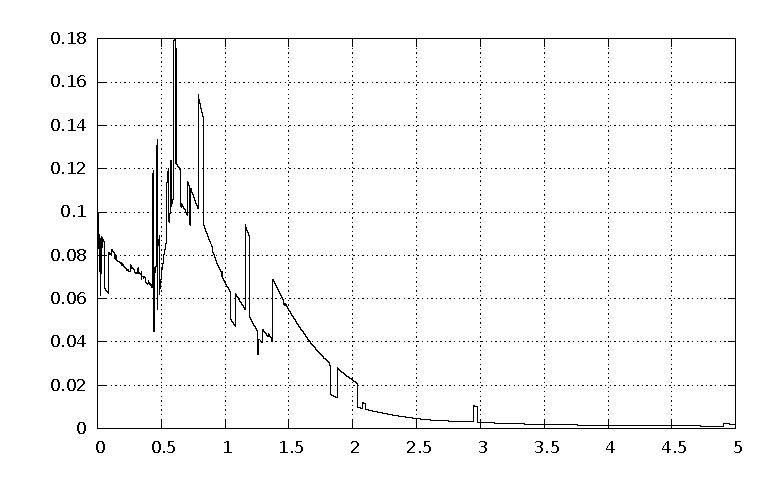
\includegraphics[width=.45\textwidth]
  {figures/nonuniform_bubble_velocity_32_both.ps}
  \caption{($\mu=\gamma=1$) $\|\vec U^m\|_{L^\infty(\Omega)}$ evolution of a
non uniform circle formed by 32 vertices with $C_s=1$ and $C_r=3$ for the
P2--P0 element, uniform mesh.}
  \label{fig:nonuniform_bubble_velocity_32_both}
\end{figure}

Instead, in Figure~\ref{fig:nonuniform_bubble_64_coarse_smooth} are shown some
snapshots of the mesh evolution when an adaptive mesh with characteristic length
$c_l=0.25$ for the boundary and 64 points on the interface is used and no
remeshing is performed. In
Figure~\ref{fig:nonuniform_bubble_velocity_64_coarse_smooth} is shown the
evolution of $\|\vec U^m\|_{L^\infty(\Omega)}$. Also in this case, the
approximations $\Gamma^m$ converge towards an equidistributed circle, while
$\vec U^m$ converges to zero.
\begin{figure}[htbp]
  \centering
  \subfloat[$t=0$]{\includegraphics[width=.45\textwidth]
  {figures/nonuniform_bubble_64_coarse_smooth_000.ps}}\\
  \subfloat[$t=0.5$]{\includegraphics[width=.45\textwidth]
  {figures/nonuniform_bubble_64_coarse_smooth_050.ps}}\quad
  \subfloat[$t=1$]{\includegraphics[width=.45\textwidth]
  {figures/nonuniform_bubble_64_coarse_smooth_100.ps}}\\
  \subfloat[$t=2.5$]{\includegraphics[width=.45\textwidth]
  {figures/nonuniform_bubble_64_coarse_smooth_250.ps}}\quad
  \subfloat[$t=5$]{\includegraphics[width=.45\textwidth]
  {figures/nonuniform_bubble_64_coarse_smooth_500.ps}}\\
  \caption{($\mu=\gamma=1$) Mesh evolution of a non uniform circle formed by
32 vertices with $C_s=1$ and no remeshing for the P2--P0 element, adaptive
mesh.}
  \label{fig:nonuniform_bubble_64_coarse_smooth}
\end{figure}

\begin{figure}[htbp]
  \centering
  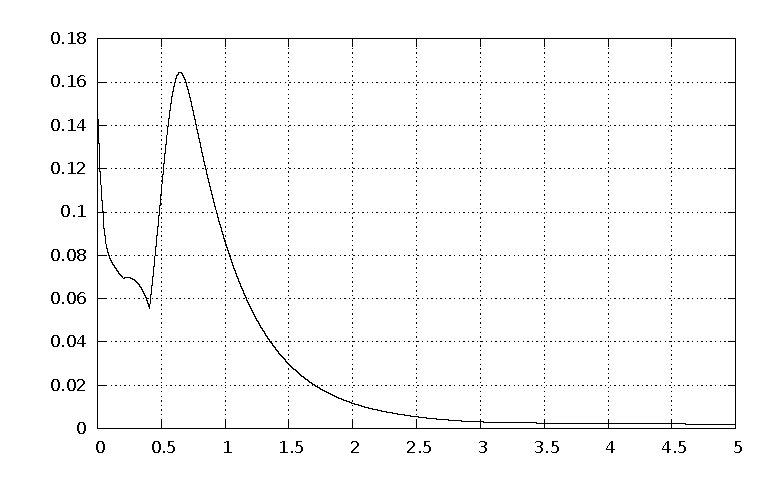
\includegraphics[width=.45\textwidth]
  {figures/nonuniform_bubble_velocity_64_coarse_smooth.ps}
  \caption{($\mu=\gamma=1$) $\|\vec U^m\|_{L^\infty(\Omega)}$ evolution of a
non uniform circle formed by 32 vertices with $C_s=1$ and no remeshing for the
P2--P0 element, adaptive mesh.}
  \label{fig:nonuniform_bubble_velocity_64_coarse_smooth}
\end{figure}

In Figure~\ref{fig:ellipse_both} is reported the pressure evolution of an
ellipse, of axis 0.8 and 0.375, with initial characteristic length $c_l=0.1$,
smoothing coefficient $C_s=1$ and remeshing coefficient $C_r=3$ for the P2--P0
element. We fix the usual domain $\Omega = (-1,1)^2$ and we use the parameters
$\mu=1$, $\gamma=1$, $\tau=10^{-2}$ and $T=10$. The mesh is uniform and we
prescribe homogeneous Dirichlet boundary condition.
Figure~\ref{fig:ellipse_both_volumes} shows the evolution of the bulk inner
relative volume
$\frac{\mathcal{L}^d(\Omega^h_-(t))}{\mathcal{L}^d(\Omega^h_-(0))}$ and the
evolution of the interface length $\mathcal{H}^{d-1}(\Gamma^h(t))$. We point out
that, since there is no exact solution to the problem, we cannot show the
pressure state at $t=0$ therefore we show the pressure state at $t=10^{-5}$.
\begin{figure}[htbp]
  \centering
  \subfloat[$t=10^{-5}$]{\includegraphics[width=.45\textwidth]
  {figures/ellipse_both_000.ps}}\\
  \subfloat[$t=2.5$]{\includegraphics[width=.45\textwidth]
  {figures/ellipse_both_250.ps}}\quad
  \subfloat[$t=5$]{\includegraphics[width=.45\textwidth]
  {figures/ellipse_both_500.ps}}\\
  \subfloat[$t=7.5$]{\includegraphics[width=.45\textwidth]
  {figures/ellipse_both_750.ps}}\quad
  \subfloat[$t=10$]{\includegraphics[width=.45\textwidth]
  {figures/ellipse_both_1000.ps}}\\
  \caption{($\mu=\gamma=1$) Pressure evolution of an ellipse with $c_l=0.1$,
$C_s=1$ and $C_r=3$ for the P2--P0 element, uniform mesh.}
  \label{fig:ellipse_both}
\end{figure}

\begin{figure}[htbp]
  \centering
  \subfloat[$\frac{\mathcal{L}^d(\Omega^h_-(t))}{\mathcal{L}^d(\Omega^h_-(0))}$]
  {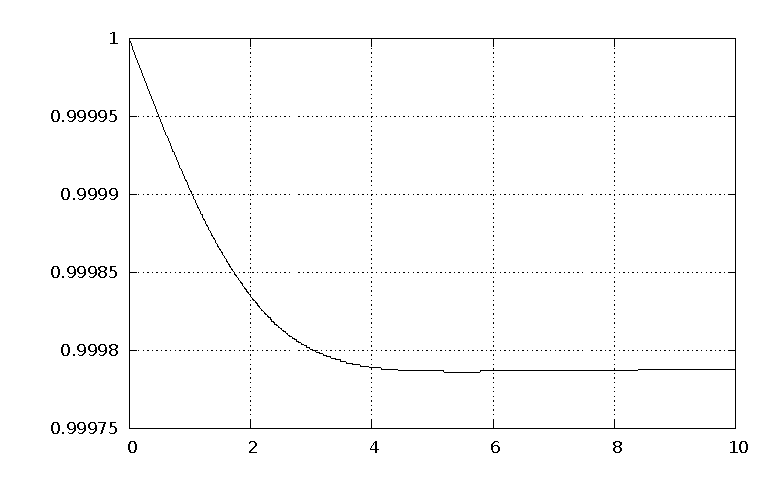
\includegraphics[width=.45\textwidth]
  {figures/ellipse_both_bulk_inner_volume.ps }}
  \subfloat[$\mathcal{H}^{d-1}(\Gamma^h(t))$]
  {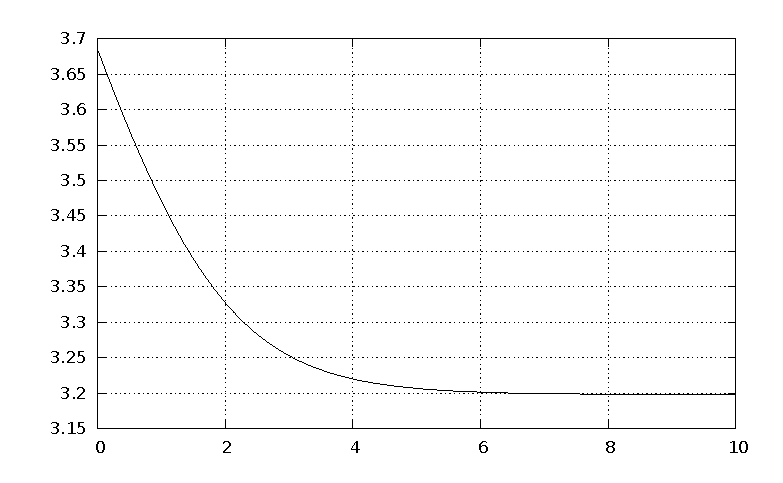
\includegraphics[width=.45\textwidth]
  {figures/ellipse_both_interface_length.ps}}
  \caption{($\mu=\gamma=1$) Bulk inner relative volume evolution and interface
length evolution of an ellipse with $c_l=0.1$, $C_s=1$ and $C_r=3$ for the
P2--P0 element, uniform mesh.}
  \label{fig:ellipse_both_volumes}
\end{figure}

Instead, in Figure~\ref{fig:ellipse_smooth} only the smoothing is used while
the evolution of the bulk inner relative volume and the evolution of the
interface length are shown in Figure~\ref{fig:ellipse_smooth_volumes}.
\begin{figure}[htbp]
  \centering
  \subfloat[$t=10^{-5}$]{\includegraphics[width=.45\textwidth]
  {figures/ellipse_smooth_000.ps}}\\
  \subfloat[$t=2.5$]{\includegraphics[width=.45\textwidth]
  {figures/ellipse_smooth_250.ps}}\quad
  \subfloat[$t=5$]{\includegraphics[width=.45\textwidth]
  {figures/ellipse_smooth_500.ps}}\\
  \subfloat[$t=7.5$]{\includegraphics[width=.45\textwidth]
  {figures/ellipse_smooth_750.ps}}\quad
  \subfloat[$t=10$]{\includegraphics[width=.45\textwidth]
  {figures/ellipse_smooth_1000.ps}}\\
  \caption{($\mu=\gamma=1$) Pressure evolution of an ellipse with $c_l=0.1$,
$C_s=1$ and no remeshing for the P2--P0 element, uniform mesh.}
  \label{fig:ellipse_smooth}
\end{figure}

\begin{figure}[htbp]
  \centering
  \subfloat[$\frac{\mathcal{L}^d(\Omega^h_-(t))}{\mathcal{L}^d(\Omega^h_-(0))}$]
  {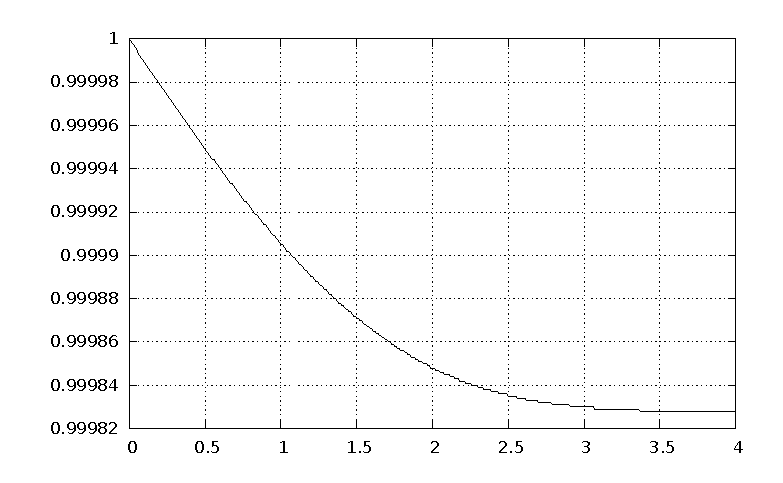
\includegraphics[width=.45\textwidth]
  {figures/ellipse_smooth_bulk_inner_volume.ps}}
  \subfloat[$\mathcal{H}^{d-1}(\Gamma^h(t))$]
  {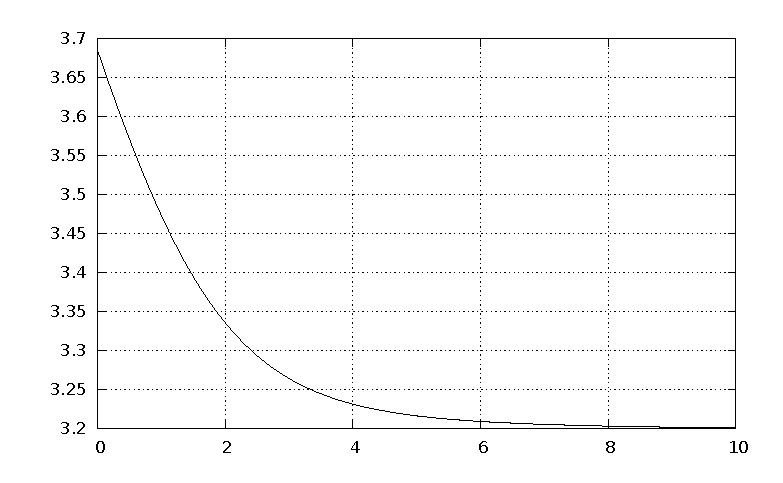
\includegraphics[width=.45\textwidth]
  {figures/ellipse_smooth_interface_length.ps}}
  \caption{($\mu=\gamma=1$) Bulk inner relative volume evolution and interface
length evolution of an ellipse with $c_l=0.1$, $C_s=1$ and no remeshing for the
P2--P0 element, uniform mesh.}
  \label{fig:ellipse_smooth_volumes}
\end{figure}





In order to choose the better remeshing coefficient $C_r$ several experiment
were carried out. Some errors for our approximation are shown in
Table~\ref{tab:expandingbubble2Dp2p0bothdiffcr} with a starting characteristic
length $c_l=0.1$, using P2--P0 polynomials and smoothing coefficient $C_s=1$.
The better result are obtained with $C_r=3$ because it reduces the number of
remeshing compared to $C_r=2$ while keeping the same performance and error
quality. For this reason we are going to use this parameter for the other
simulations.
\begin{table*}
 \center
\begin{tabular}{llHllHll}
\hline
$C_r$ & $\errorXx$ & $\LerrorUu2$ & $\errorUu2$ & $\LerrorPp$ & $\errorPp0$ &
$CPU[s]$ & $K_\Omega^T$\\
\hline
2 & 1.46658e-03 & 1.05801e-04 & 8.73227e-04 & 2.14589e-01 & 3.68834e-02 & 4297
& 452\\
3 & 1.47162e-03 & 1.02085e-04 & 7.19650e-04 & 2.13599e-01 & 3.68834e-02 & 3919
& 468\\
4 & 1.46761e-03 & 1.27330e-04 & 8.55458e-04 & 2.19071e-01 & 3.68834e-02 & 4682
& 504\\
5 & 1.47218e-03 & 1.26419e-04 & 7.20711e-04 & 2.12456e-01 & 3.68834e-02 & 4775&
468\\
\hline
\end{tabular}
\caption{($\mu_+ = 10\,\mu_- = \gamma = 1,\alpha = 0.15$) Expanding bubble
problem on $(-1,1)^2\setminus[-\frac{1}{3},\frac{1}{3}]^2$ over the time
interval $[0,1]$ for the P2--P0 element, $C_s=1$, $c_l=0.1$ and uniform mesh.}
\label{tab:expandingbubble2Dp2p0bothdiffcr}
\end{table*}

In all the previous simulations, the meshes used were uniform therefore the
characteristic length was equal for all the nodes. Moreover they were kept
uniform also after the remeshing. Obviously, with this approach, it is very
expensive to have a large number of interface elements since it leads to a
drastic increase of bulk elements. In the following simulations, instead, we use
adaptive meshes which are fine close to the interface and coarse far from the
interface.





Finally, we report a shear flow in the domain $\Omega=(-1,1)^2$, with a circle
of radius $r=0.5$ as initial interface. We prescribe the inhomogeneous Dirichlet
boundary condition
\begin{equation*}
\vec g(\vec z)=(z_2,0)^T\quad \mbox{on }\partial\Omega\,,
\end{equation*}
and we use the parameters $\mu=1$, $\gamma=3$, $\tau=10^{-2}$ and $T=5$. In
Figure~\ref{fig:shear_2d} is reported the pressure evolution using a
characteristic length $c_l=0.05$ and an uniform mesh, smoothing coefficient
$C_s=1$ and remeshing coefficient $C_r=3$ for the P2--P0 element. In
Figure~\ref{fig:shear_2d_velocity} is shown the velocity vector field evolution
while the bulk inner relative volume evolution
$\frac{\mathcal{L}^d(\Omega^h_-(t))}{\mathcal{L}^d(\Omega^h_-(0))}$ is reported
in Figure~\ref{fig:shear_2d_bulk_inner_volume}.
\begin{figure}[htbp]
  \centering
  \subfloat[$t=0.5$]{\includegraphics[width=.45\textwidth]
  {figures/2d_shear_050.ps}}\quad
  \subfloat[$t=1$]{\includegraphics[width=.45\textwidth]
  {figures/2d_shear_100.ps}}\\
  \subfloat[$t=2.5$]{\includegraphics[width=.45\textwidth]
  {figures/2d_shear_250.ps}}\quad
  \subfloat[$t=5$]{\includegraphics[width=.45\textwidth]
  {figures/2d_shear_500.ps}}\\
 \caption{($\mu=1,\gamma=3$) Pressure evolution of the 2D shear flow with
$c_l=0.05$, $C_s=1$ and $C_r=3$ for the P2--P0 element, uniform mesh.}
  \label{fig:shear_2d}
\end{figure}

\begin{figure}[htbp]
  \centering
  \subfloat[$t=0.5$]{\includegraphics[width=.45\textwidth]
  {figures/2d_shear_velocity_050.ps}}\quad
  \subfloat[$t=1$]{\includegraphics[width=.45\textwidth]
  {figures/2d_shear_velocity_100.ps}}\\
  \subfloat[$t=2.5$]{\includegraphics[width=.45\textwidth]
  {figures/2d_shear_velocity_250.ps}}\quad
  \subfloat[$t=5$]{\includegraphics[width=.45\textwidth]
  {figures/2d_shear_velocity_500.ps}}\\
  \caption{($\mu=1,\gamma=3$) Velocity vector field of the 2D shear flow with
$c_l=0.05$, $C_s=1$ and $C_r=3$ for the P2--P0 element, uniform mesh.}
  \label{fig:shear_2d_velocity}
\end{figure}

\begin{figure}[htbp]
  \centering
  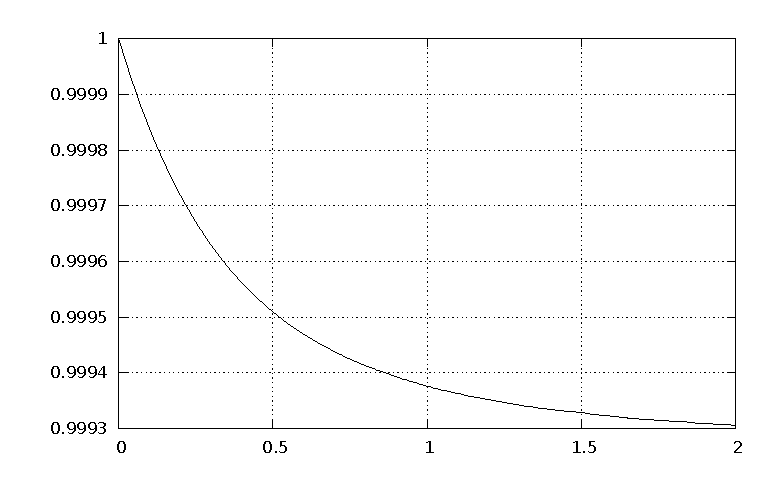
\includegraphics[width=.45\textwidth]{figures/2d_shear_bulk_inner_volume.ps}
  \caption{($\mu=\gamma=1$) Bulk inner relative volume evolution of the 2D
shear flow with $c_l=0.05$, $C_s=1$ and $C_r=3$ for the P2--P0 element, uniform
mesh.}
  \label{fig:shear_2d_bulk_inner_volume}
\end{figure}

Instead, in Figure~\ref{fig:shear_2d_smooth} the remeshing coefficient is
$C_r=0$ so only the smoothing is used. The bulk inner relative volume evolution
is reported in Figure~\ref{fig:shear_2d_smooth_bulk_inner_volume}.
\begin{figure}[htbp]
  \centering
  \subfloat[$t=0.5$]{\includegraphics[width=.45\textwidth]
  {figures/2d_shear_smooth_050.ps}}\quad
  \subfloat[$t=1$]{\includegraphics[width=.45\textwidth]
  {figures/2d_shear_smooth_100.ps}}\\
  \subfloat[$t=2.5$]{\includegraphics[width=.45\textwidth]
  {figures/2d_shear_smooth_250.ps}}\quad
  \subfloat[$t=5$]{\includegraphics[width=.45\textwidth]
  {figures/2d_shear_smooth_500.ps}}\\
  \caption{($\mu=1,\gamma=3$) Pressure evolution of the 2D shear flow with
$c_l=0.05$, $C_s=1$ and no remeshing for the P2--P0 element, uniform mesh.}
  \label{fig:shear_2d_smooth}
\end{figure}

\begin{figure}[htbp]
  \centering
  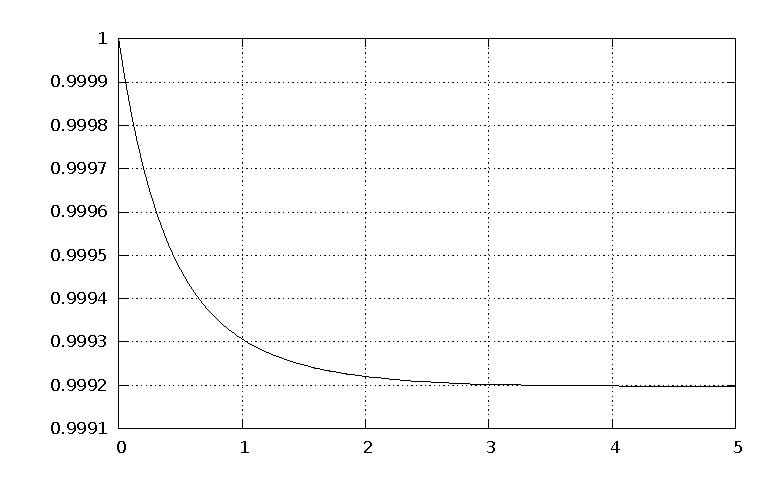
\includegraphics[width=.45\textwidth]
  {figures/2d_shear_smooth_bulk_inner_volume.ps}
  \caption{($\mu=\gamma=1$) Bulk inner relative volume evolution of the 2D
shear flow with $c_l=0.05$, $C_s=1$ and no remeshing for the P2--P0 element,
uniform mesh.}
  \label{fig:shear_2d_smooth_bulk_inner_volume}
\end{figure}

\subsection{Numerical results in 3d} \label{subsec:numerical_results_3d}

For the stationary bubble test we use the domain $\Omega = (-1,1)^3$ and we
choose, for the true solution (\ref{eq:radialr},b), the parameters
\begin{equation*}
\mu = \gamma = 1\,.
\end{equation*}
Therefore, the true solution reduces to $r(t) = \frac{1}{2}$, $\vec u(\cdot, t)
= \vec 0$ and $p(t) = 4\,\charfcn{\Omega_-(0)} - \frac{\pi}{12}$ for all
$t\geq0$.

In Table~\ref{tab:bubble3Delements} it is reported the characteristic length
$c_l$, which prescribes the desired size of the elements, used to create the
mesh for the stationary bubble problem, the corresponding number of interface
elements $K_\Gamma$ generated, the corresponding number of bulk elements
$K_\Omega$ generated and the time step $\tau$ used. The interface mesh is
obtained applying a surface diffusion to a sphere until the surface is
stationary which means until the displacement is 0 up to machine accuracy for
all the nodes. The bulk mesh is uniform.
\begin{table*}
 \center
\begin{tabular}{llll}
\hline
$c_l$ & $K_\Gamma$ & $K_\Omega$ & $\tau$ \\
\hline
0.5 & 32 & 408 & $10^{-2}$ \\
0.25 & 220 & 3590 & $10^{-2}$\\
0.125 & 596 & 20473 & $10^{-2}$\\
\hline
\end{tabular}
\caption{Number of interface elements ($K_\Gamma$), number of bulk elements
($K_\Omega$) and time step ($\tau$) for a certain characteristic length ($c_l$)
for the 3D stationary bubble problem, stationary uniform mesh.}
\label{tab:bubble3Delements}
\end{table*}

Since the solution is stationary, neither smoothing nor remeshing is performed.


We see that the radius error in Table~\ref{tab:bubble3Dp2p0} is terrible
compared to the analogous test in 2D. The reason is that in 2D the initial
discrete interface is equidistributed and its radius is exactly 0.5 while in 3D
the mesh is equidistributed but the initial radius has already an error. This
error is exactly the one seen in the table since the displacement is always 0 up
to machine accuracy.

Finally, we report a shear flow in the domain $\Omega=(-1,1)^3$, with a sphere
of radius $r=0.5$ as initial interface. The initial interface mesh is a
non-stationary sphere while the bulk mesh is uniform. We prescribe the
inhomogeneous Dirichlet boundary condition
\begin{equation*}
\vec g(\vec z)=(z_3,0,0)^T\quad \mbox{on }\partial\Omega\,,
\end{equation*}
and we use the parameters $\mu=1$, $\gamma=3$, $\tau=10^{-2}$ and $T=5$. In
Figure~\ref{fig:shear_3d} is reported the interface evolution of the sphere with
initial characteristic length $c_l=0.125$, smoothing coefficient $C_s=1$ and
remeshing coefficient $C_r=3$ for the P2--P0 element. The characteristic length
for the boundary is fixed and not uniform like in the 2D case. In
Figure~\ref{fig:shear_3d_velocity} is shown the velocity vector field evolution
in the plane normal to $(0,1,0)$ and passing through the origin while the bulk
inner relative volume evolution
$\frac{\mathcal{L}^d(\Omega^h_-(t))}{\mathcal{L}^d(\Omega^h_-(0))}$ is reported
in Figure~\ref{fig:shear_3d_bulk_inner_volume}.
\begin{figure}[htbp]
  \centering
  \subfloat[$t=0$]{\includegraphics[width=.45\textwidth]
  {figures/3d_shear_000.ps}}\\
  \subfloat[$t=0.5$]{\includegraphics[width=.45\textwidth]
  {figures/3d_shear_050.ps}}\quad
  \subfloat[$t=1$]{\includegraphics[width=.45\textwidth]
  {figures/3d_shear_100.ps}}\\
  \subfloat[$t=2.5$]{\includegraphics[width=.45\textwidth]
  {figures/3d_shear_250.ps}}\quad
  \subfloat[$t=5$]{\includegraphics[width=.45\textwidth]
  {figures/3d_shear_500.ps}}\\
  \caption{($\mu=1,\gamma=3$) Interface evolution of the 3D shear flow with
$c_l=0.125$, $C_s=1$ and $C_r=3$ for the P2--P0 element, uniform mesh.}
  \label{fig:shear_3d}
\end{figure}

\begin{figure}[htbp]
  \centering
  \subfloat[$t=0.5$]{\includegraphics[width=.45\textwidth]
  {figures/3d_shear_velocity_050.ps}}\quad
  \subfloat[$t=1$]{\includegraphics[width=.45\textwidth]
  {figures/3d_shear_velocity_100.ps}}\\
  \subfloat[$t=2.5$]{\includegraphics[width=.45\textwidth]
  {figures/3d_shear_velocity_250.ps}}\quad
  \subfloat[$t=5$]{\includegraphics[width=.45\textwidth]
  {figures/3d_shear_velocity_500.ps}}\\
  \caption{($\mu=1,\gamma=3$) Velocity vector field in the plane normal to
$(0,1,0)$ and passing through the origin of the 3D shear flow with $c_l=0.125$,
$C_s=1$ and $C_r=3$ for the P2--P0 element, uniform mesh.}
  \label{fig:shear_3d_velocity}
\end{figure}

\begin{figure}[htbp]
  \centering
  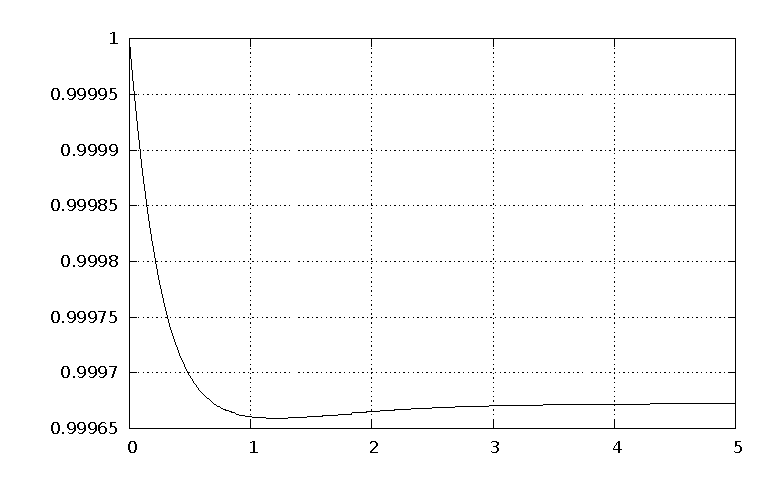
\includegraphics[width=.45\textwidth]{figures/3d_shear_bulk_inner_volume.ps}
 \caption{($\mu=\gamma=1$) Bulk inner relative volume evolution of the 3D
shear flow with $c_l=0.125$, $C_s=1$ and $C_r=3$ for the P2--P0 element,
uniform mesh.}
  \label{fig:shear_3d_bulk_inner_volume}
\end{figure}

\section{Conclusion}\label{sec:conclusion}
\textcolor{magenta}{TODO : add comparison reults unfitted scheme scheme stokes
paper}

The P2--P0 element has the same accuracy of the P2--(P1+P0) element but it is
simpler to implement, always satisfies the LBB condition and the resulting
linear system is smaller therefore it is the best choice.

The adaptive mesh works very well for the stationary bubble problem. Indeed,
with a fraction of bulk elements, it reaches the same accuracy of the uniform
mesh. Unfortunately this is not the case for the expanding bubble problem. For
this problem, the uniform mesh is much faster and requires less bulk elements
compared to the adaptive mesh therefore.\footnote{But they have different
$\tau$!}

In the 2D expanding bubble problem, We can observe that the simulations which
use only the smoothing have bigger errors and take more time therefore it is not
feasible to use only the smoothing process. On the other side both only
remeshing and smoothing/remeshing combined achieve almost the same quality and
performance. It is important to notice that the performance are almost the same
for sequential code (our case) but in parallel computation the remeshing is the
real bottleneck therefore it is way better to use the combined
smoothing/remeshing approach.

Both element capture perfectly the jump in the pressure.
\newpage
\bibliographystyle{siam}
\bibliography{../bib/robert_refs,../bib/marco_refs}
\end{document}
